% Options for packages loaded elsewhere
% Options for packages loaded elsewhere
\PassOptionsToPackage{unicode}{hyperref}
\PassOptionsToPackage{hyphens}{url}
%
\documentclass[
  english,
  letterpaper,
]{scrbook}
\usepackage{xcolor}
\usepackage{amsmath,amssymb}
\setcounter{secnumdepth}{5}
\usepackage{iftex}
\ifPDFTeX
  \usepackage[T1]{fontenc}
  \usepackage[utf8]{inputenc}
  \usepackage{textcomp} % provide euro and other symbols
\else % if luatex or xetex
  \usepackage{unicode-math} % this also loads fontspec
  \defaultfontfeatures{Scale=MatchLowercase}
  \defaultfontfeatures[\rmfamily]{Ligatures=TeX,Scale=1}
\fi
\usepackage{lmodern}
\ifPDFTeX\else
  % xetex/luatex font selection
\fi
% Use upquote if available, for straight quotes in verbatim environments
\IfFileExists{upquote.sty}{\usepackage{upquote}}{}
\IfFileExists{microtype.sty}{% use microtype if available
  \usepackage[]{microtype}
  \UseMicrotypeSet[protrusion]{basicmath} % disable protrusion for tt fonts
}{}
\makeatletter
\@ifundefined{KOMAClassName}{% if non-KOMA class
  \IfFileExists{parskip.sty}{%
    \usepackage{parskip}
  }{% else
    \setlength{\parindent}{0pt}
    \setlength{\parskip}{6pt plus 2pt minus 1pt}}
}{% if KOMA class
  \KOMAoptions{parskip=half}}
\makeatother
% Make \paragraph and \subparagraph free-standing
\makeatletter
\ifx\paragraph\undefined\else
  \let\oldparagraph\paragraph
  \renewcommand{\paragraph}{
    \@ifstar
      \xxxParagraphStar
      \xxxParagraphNoStar
  }
  \newcommand{\xxxParagraphStar}[1]{\oldparagraph*{#1}\mbox{}}
  \newcommand{\xxxParagraphNoStar}[1]{\oldparagraph{#1}\mbox{}}
\fi
\ifx\subparagraph\undefined\else
  \let\oldsubparagraph\subparagraph
  \renewcommand{\subparagraph}{
    \@ifstar
      \xxxSubParagraphStar
      \xxxSubParagraphNoStar
  }
  \newcommand{\xxxSubParagraphStar}[1]{\oldsubparagraph*{#1}\mbox{}}
  \newcommand{\xxxSubParagraphNoStar}[1]{\oldsubparagraph{#1}\mbox{}}
\fi
\makeatother

\usepackage{color}
\usepackage{fancyvrb}
\newcommand{\VerbBar}{|}
\newcommand{\VERB}{\Verb[commandchars=\\\{\}]}
\DefineVerbatimEnvironment{Highlighting}{Verbatim}{commandchars=\\\{\}}
% Add ',fontsize=\small' for more characters per line
\usepackage{framed}
\definecolor{shadecolor}{RGB}{241,243,245}
\newenvironment{Shaded}{\begin{snugshade}}{\end{snugshade}}
\newcommand{\AlertTok}[1]{\textcolor[rgb]{0.68,0.00,0.00}{#1}}
\newcommand{\AnnotationTok}[1]{\textcolor[rgb]{0.37,0.37,0.37}{#1}}
\newcommand{\AttributeTok}[1]{\textcolor[rgb]{0.40,0.45,0.13}{#1}}
\newcommand{\BaseNTok}[1]{\textcolor[rgb]{0.68,0.00,0.00}{#1}}
\newcommand{\BuiltInTok}[1]{\textcolor[rgb]{0.00,0.23,0.31}{#1}}
\newcommand{\CharTok}[1]{\textcolor[rgb]{0.13,0.47,0.30}{#1}}
\newcommand{\CommentTok}[1]{\textcolor[rgb]{0.37,0.37,0.37}{#1}}
\newcommand{\CommentVarTok}[1]{\textcolor[rgb]{0.37,0.37,0.37}{\textit{#1}}}
\newcommand{\ConstantTok}[1]{\textcolor[rgb]{0.56,0.35,0.01}{#1}}
\newcommand{\ControlFlowTok}[1]{\textcolor[rgb]{0.00,0.23,0.31}{\textbf{#1}}}
\newcommand{\DataTypeTok}[1]{\textcolor[rgb]{0.68,0.00,0.00}{#1}}
\newcommand{\DecValTok}[1]{\textcolor[rgb]{0.68,0.00,0.00}{#1}}
\newcommand{\DocumentationTok}[1]{\textcolor[rgb]{0.37,0.37,0.37}{\textit{#1}}}
\newcommand{\ErrorTok}[1]{\textcolor[rgb]{0.68,0.00,0.00}{#1}}
\newcommand{\ExtensionTok}[1]{\textcolor[rgb]{0.00,0.23,0.31}{#1}}
\newcommand{\FloatTok}[1]{\textcolor[rgb]{0.68,0.00,0.00}{#1}}
\newcommand{\FunctionTok}[1]{\textcolor[rgb]{0.28,0.35,0.67}{#1}}
\newcommand{\ImportTok}[1]{\textcolor[rgb]{0.00,0.46,0.62}{#1}}
\newcommand{\InformationTok}[1]{\textcolor[rgb]{0.37,0.37,0.37}{#1}}
\newcommand{\KeywordTok}[1]{\textcolor[rgb]{0.00,0.23,0.31}{\textbf{#1}}}
\newcommand{\NormalTok}[1]{\textcolor[rgb]{0.00,0.23,0.31}{#1}}
\newcommand{\OperatorTok}[1]{\textcolor[rgb]{0.37,0.37,0.37}{#1}}
\newcommand{\OtherTok}[1]{\textcolor[rgb]{0.00,0.23,0.31}{#1}}
\newcommand{\PreprocessorTok}[1]{\textcolor[rgb]{0.68,0.00,0.00}{#1}}
\newcommand{\RegionMarkerTok}[1]{\textcolor[rgb]{0.00,0.23,0.31}{#1}}
\newcommand{\SpecialCharTok}[1]{\textcolor[rgb]{0.37,0.37,0.37}{#1}}
\newcommand{\SpecialStringTok}[1]{\textcolor[rgb]{0.13,0.47,0.30}{#1}}
\newcommand{\StringTok}[1]{\textcolor[rgb]{0.13,0.47,0.30}{#1}}
\newcommand{\VariableTok}[1]{\textcolor[rgb]{0.07,0.07,0.07}{#1}}
\newcommand{\VerbatimStringTok}[1]{\textcolor[rgb]{0.13,0.47,0.30}{#1}}
\newcommand{\WarningTok}[1]{\textcolor[rgb]{0.37,0.37,0.37}{\textit{#1}}}

\usepackage{longtable,booktabs,array}
\newcounter{none} % for unnumbered tables
\usepackage{calc} % for calculating minipage widths
% Correct order of tables after \paragraph or \subparagraph
\usepackage{etoolbox}
\makeatletter
\patchcmd\longtable{\par}{\if@noskipsec\mbox{}\fi\par}{}{}
\makeatother
% Allow footnotes in longtable head/foot
\IfFileExists{footnotehyper.sty}{\usepackage{footnotehyper}}{\usepackage{footnote}}
\makesavenoteenv{longtable}
\usepackage{graphicx}
\makeatletter
\newsavebox\pandoc@box
\newcommand*\pandocbounded[1]{% scales image to fit in text height/width
  \sbox\pandoc@box{#1}%
  \Gscale@div\@tempa{\textheight}{\dimexpr\ht\pandoc@box+\dp\pandoc@box\relax}%
  \Gscale@div\@tempb{\linewidth}{\wd\pandoc@box}%
  \ifdim\@tempb\p@<\@tempa\p@\let\@tempa\@tempb\fi% select the smaller of both
  \ifdim\@tempa\p@<\p@\scalebox{\@tempa}{\usebox\pandoc@box}%
  \else\usebox{\pandoc@box}%
  \fi%
}
% Set default figure placement to htbp
\def\fps@figure{htbp}
\makeatother


% definitions for citeproc citations
\NewDocumentCommand\citeproctext{}{}
\NewDocumentCommand\citeproc{mm}{%
  \begingroup\def\citeproctext{#2}\cite{#1}\endgroup}
\makeatletter
 % allow citations to break across lines
 \let\@cite@ofmt\@firstofone
 % avoid brackets around text for \cite:
 \def\@biblabel#1{}
 \def\@cite#1#2{{#1\if@tempswa , #2\fi}}
\makeatother
\newlength{\cslhangindent}
\setlength{\cslhangindent}{1.5em}
\newlength{\csllabelwidth}
\setlength{\csllabelwidth}{3em}
\newenvironment{CSLReferences}[2] % #1 hanging-indent, #2 entry-spacing
 {\begin{list}{}{%
  \setlength{\itemindent}{0pt}
  \setlength{\leftmargin}{0pt}
  \setlength{\parsep}{0pt}
  % turn on hanging indent if param 1 is 1
  \ifodd #1
   \setlength{\leftmargin}{\cslhangindent}
   \setlength{\itemindent}{-1\cslhangindent}
  \fi
  % set entry spacing
  \setlength{\itemsep}{#2\baselineskip}}}
 {\end{list}}
\usepackage{calc}
\newcommand{\CSLBlock}[1]{\hfill\break\parbox[t]{\linewidth}{\strut\ignorespaces#1\strut}}
\newcommand{\CSLLeftMargin}[1]{\parbox[t]{\csllabelwidth}{\strut#1\strut}}
\newcommand{\CSLRightInline}[1]{\parbox[t]{\linewidth - \csllabelwidth}{\strut#1\strut}}
\newcommand{\CSLIndent}[1]{\hspace{\cslhangindent}#1}

\ifLuaTeX
\usepackage[bidi=basic,shorthands=off]{babel}
\else
\usepackage[bidi=default,shorthands=off]{babel}
\fi
\ifLuaTeX
  \usepackage{selnolig} % disable illegal ligatures
\fi


\setlength{\emergencystretch}{3em} % prevent overfull lines

\providecommand{\tightlist}{%
  \setlength{\itemsep}{0pt}\setlength{\parskip}{0pt}}



 


\makeatletter
\@ifpackageloaded{tcolorbox}{}{\usepackage[skins,breakable]{tcolorbox}}
\@ifpackageloaded{fontawesome5}{}{\usepackage{fontawesome5}}
\definecolor{quarto-callout-color}{HTML}{909090}
\definecolor{quarto-callout-note-color}{HTML}{0758E5}
\definecolor{quarto-callout-important-color}{HTML}{CC1914}
\definecolor{quarto-callout-warning-color}{HTML}{EB9113}
\definecolor{quarto-callout-tip-color}{HTML}{00A047}
\definecolor{quarto-callout-caution-color}{HTML}{FC5300}
\definecolor{quarto-callout-color-frame}{HTML}{acacac}
\definecolor{quarto-callout-note-color-frame}{HTML}{4582ec}
\definecolor{quarto-callout-important-color-frame}{HTML}{d9534f}
\definecolor{quarto-callout-warning-color-frame}{HTML}{f0ad4e}
\definecolor{quarto-callout-tip-color-frame}{HTML}{02b875}
\definecolor{quarto-callout-caution-color-frame}{HTML}{fd7e14}
\makeatother
\makeatletter
\@ifpackageloaded{bookmark}{}{\usepackage{bookmark}}
\makeatother
\makeatletter
\@ifpackageloaded{caption}{}{\usepackage{caption}}
\AtBeginDocument{%
\ifdefined\contentsname
  \renewcommand*\contentsname{Table of contents}
\else
  \newcommand\contentsname{Table of contents}
\fi
\ifdefined\listfigurename
  \renewcommand*\listfigurename{List of Figures}
\else
  \newcommand\listfigurename{List of Figures}
\fi
\ifdefined\listtablename
  \renewcommand*\listtablename{List of Tables}
\else
  \newcommand\listtablename{List of Tables}
\fi
\ifdefined\figurename
  \renewcommand*\figurename{Figure}
\else
  \newcommand\figurename{Figure}
\fi
\ifdefined\tablename
  \renewcommand*\tablename{Table}
\else
  \newcommand\tablename{Table}
\fi
}
\@ifpackageloaded{float}{}{\usepackage{float}}
\floatstyle{ruled}
\@ifundefined{c@chapter}{\newfloat{codelisting}{h}{lop}}{\newfloat{codelisting}{h}{lop}[chapter]}
\floatname{codelisting}{Listing}
\newcommand*\listoflistings{\listof{codelisting}{List of Listings}}
\makeatother
\makeatletter
\makeatother
\makeatletter
\@ifpackageloaded{caption}{}{\usepackage{caption}}
\@ifpackageloaded{subcaption}{}{\usepackage{subcaption}}
\makeatother
\usepackage{bookmark}
\IfFileExists{xurl.sty}{\usepackage{xurl}}{} % add URL line breaks if available
\urlstyle{same}
% fallback for those not using the hyperref driver hyperxmp:
\makeatletter
\@ifundefined{xmpquote}{\newcommand{\xmpquote}[1]{#1}}{}
\makeatother
\hypersetup{
  pdftitle={Acoustic Measures of Voice Quality},
  pdfauthor={Jorge C. Lucero},
  pdflang={en},
  hidelinks,
  pdfcreator={LaTeX via pandoc}}


\title{Acoustic Measures of Voice Quality}
\usepackage{etoolbox}
\makeatletter
\providecommand{\subtitle}[1]{% add subtitle to \maketitle
  \apptocmd{\@title}{\par {\large #1 \par}}{}{}
}
\makeatother
\subtitle{A Living Reference}
\author{Jorge C. Lucero}
\date{2026-09-20}
\begin{document}
\frontmatter
\maketitle

\renewcommand*\contentsname{Table of contents}
{
\setcounter{tocdepth}{2}
\tableofcontents
}

\mainmatter
\bookmarksetup{startatroot}

\chapter*{Preface}\label{preface}
\addcontentsline{toc}{chapter}{Preface}

\markboth{Preface}{Preface}

\emph{Acoustic Measures of Voice Quality} is an open, \textbf{living
reference} on how the acoustic measures used in voice assessment are
computed and interpreted. It is written for speech-language
pathologists, voice scientists, and students who want to understand not
just \emph{what} a number like CPPS or AVQI is, but \emph{how} it is
derived from the signal, what it captures, where it fails, and how to
read it in practice.

Unlike a printed textbook, this reference is versioned and continuously
updated. Each release is archived with its own DOI, so you can cite a
specific, frozen version while the living site continues to improve.

\section*{How to cite}\label{how-to-cite}
\addcontentsline{toc}{section}{How to cite}

\markright{How to cite}

\begin{quote}
Lucero, J. C. (2026). \emph{Acoustic Measures of Voice Quality: A Living
Reference} (Version 0.0.1). Zenodo.
https://doi.org/10.5281/zenodo.22739050
\end{quote}

\section*{License}\label{license}
\addcontentsline{toc}{section}{License}

\markright{License}

The prose and figures are licensed under
\href{https://creativecommons.org/licenses/by/4.0/}{CC BY 4.0}; the code
examples are licensed under the
\href{https://opensource.org/licenses/MIT}{MIT License}. You are free to
share, adapt, and translate this work with attribution.

\section*{Relationship to PhonaLab}\label{relationship-to-phonalab}
\addcontentsline{toc}{section}{Relationship to PhonaLab}

\markright{Relationship to PhonaLab}

This reference is the \emph{methods} companion to
\href{https://phonalab.com}{PhonaLab}. Where this text explains what a
measure is and how it is computed, PhonaLab lets you compute it on your
own recording. Each measure chapter links to the corresponding PhonaLab
tool, and PhonaLab links back here for the underlying method.

\bookmarksetup{startatroot}

\chapter{About this reference}\label{about-this-reference}

\section{Scope}\label{scope}

This reference covers \textbf{acoustic measures of voice quality} ---
the quantities computed from a voice recording that characterize
periodicity, noise, and spectral structure. It does not cover
aerodynamic measurement, laryngeal imaging, or auditory-perceptual
assessment, except where those are needed to interpret or validate an
acoustic measure.

\section{Who this is for}\label{who-this-is-for}

The reference assumes you know what a spectrogram is and are comfortable
reading a plot. It is not an introductory speech-science text. It is
aimed at clinicians and researchers who use these measures and want to
understand them precisely enough to apply, compare, or implement them.

\section{How the measures are
organized}\label{how-the-measures-are-organized}

Measures are grouped by \textbf{what they capture}, not by algorithm
family or by the pathology they detect:

\begin{itemize}
\tightlist
\item
  \textbf{Part I --- Foundations.} The voice signal, recording quality,
  segmentation, and voicing detection: what must be true of a recording
  before any measure is trustworthy.
\item
  \textbf{Part II --- Periodicity and stability.} f0 estimation, jitter,
  shimmer, and the nonlinear dynamical measures.
\item
  \textbf{Part III --- Noise and harmonic structure.} HNR and its
  variants, GNE, CPPS, and spectral tilt measures.
\item
  \textbf{Part IV --- Composite and clinical indices.} AVQI, ABI, and
  how they are built from the Part II and Part III measures.
\item
  \textbf{Part V --- Beyond the traditional measures.}
  Machine-learning-derived features and where the field is going.
\end{itemize}

Each measure is presented with a consistent structure: definition,
computation, what it captures physiologically, known confounds,
normative ranges, validation, and a runnable example.

\part{Part I --- Foundations}

\chapter{The voice signal}\label{the-voice-signal}

\begin{tcolorbox}[enhanced jigsaw, arc=.35mm, bottomrule=.15mm, bottomtitle=1mm, breakable, colback=white, colbacktitle=quarto-callout-note-color!10!white, colframe=quarto-callout-note-color-frame, coltitle=black, left=2mm, leftrule=.75mm, opacityback=0, opacitybacktitle=0.6, rightrule=.15mm, title=\textcolor{quarto-callout-note-color}{\faInfo}\hspace{0.5em}{Note}, titlerule=0mm, toprule=.15mm, toptitle=1mm]

This is a \textbf{scaffold stub}. It exists to prove the end-to-end
pipeline --- including executable code --- renders and publishes
correctly. Replace its content when you begin writing Part I.

\end{tcolorbox}

\section{A synthetic voiced signal}\label{a-synthetic-voiced-signal}

The code cell below generates a simple harmonic-rich signal, a stand-in
for a sustained vowel, and plots a short segment. If this figure appears
in the rendered site, your Jupyter/Python execution path is working.

\begin{Shaded}
\begin{Highlighting}[]
\ImportTok{import}\NormalTok{ numpy }\ImportTok{as}\NormalTok{ np}
\ImportTok{import}\NormalTok{ matplotlib.pyplot }\ImportTok{as}\NormalTok{ plt}

\NormalTok{fs }\OperatorTok{=} \DecValTok{16000}                      \CommentTok{\# sample rate (Hz)}
\NormalTok{dur }\OperatorTok{=} \FloatTok{0.5}                       \CommentTok{\# seconds}
\NormalTok{t }\OperatorTok{=}\NormalTok{ np.linspace(}\DecValTok{0}\NormalTok{, dur, }\BuiltInTok{int}\NormalTok{(fs }\OperatorTok{*}\NormalTok{ dur), endpoint}\OperatorTok{=}\VariableTok{False}\NormalTok{)}
\NormalTok{f0 }\OperatorTok{=} \FloatTok{120.0}                      \CommentTok{\# fundamental frequency (Hz)}

\CommentTok{\# Sum of harmonics with 1/k amplitude decay}
\NormalTok{signal }\OperatorTok{=} \BuiltInTok{sum}\NormalTok{((}\FloatTok{1.0} \OperatorTok{/}\NormalTok{ k) }\OperatorTok{*}\NormalTok{ np.sin(}\DecValTok{2} \OperatorTok{*}\NormalTok{ np.pi }\OperatorTok{*}\NormalTok{ f0 }\OperatorTok{*}\NormalTok{ k }\OperatorTok{*}\NormalTok{ t) }\ControlFlowTok{for}\NormalTok{ k }\KeywordTok{in} \BuiltInTok{range}\NormalTok{(}\DecValTok{1}\NormalTok{, }\DecValTok{20}\NormalTok{))}

\NormalTok{fig, ax }\OperatorTok{=}\NormalTok{ plt.subplots(figsize}\OperatorTok{=}\NormalTok{(}\DecValTok{7}\NormalTok{, }\FloatTok{2.5}\NormalTok{))}
\NormalTok{ax.plot(t[:}\DecValTok{400}\NormalTok{], signal[:}\DecValTok{400}\NormalTok{], linewidth}\OperatorTok{=}\DecValTok{1}\NormalTok{)}
\NormalTok{ax.set\_xlabel(}\StringTok{"Time (s)"}\NormalTok{)}
\NormalTok{ax.set\_ylabel(}\StringTok{"Amplitude"}\NormalTok{)}
\NormalTok{fig.tight\_layout()}
\NormalTok{plt.show()}
\end{Highlighting}
\end{Shaded}

\begin{figure}[H]

\centering{

\pandocbounded{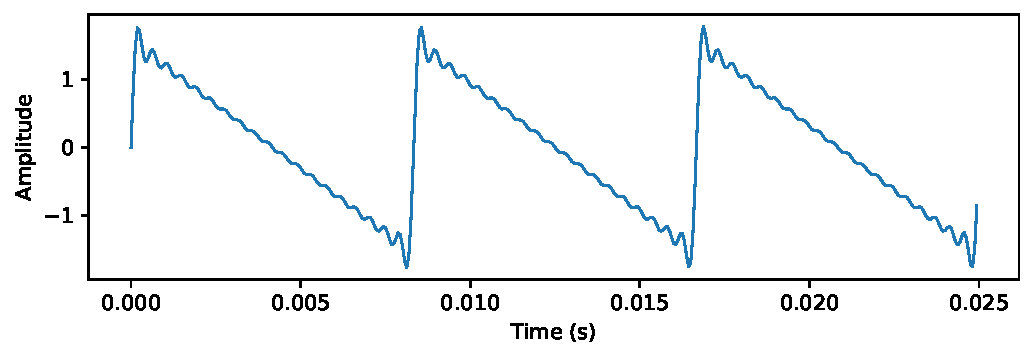
\includegraphics[keepaspectratio]{foundations-signal_files/figure-pdf/fig-synthetic-output-1.pdf}}

}

\caption{\label{fig-synthetic}A synthetic harmonic-rich signal (f0 = 120
Hz), first 25 ms.}

\end{figure}%

Once real content replaces this stub, the same executable pattern will
let every measure chapter compute and display results on real signals
--- ideally the same libraries PhonaLab uses, so the reference and the
platform stay consistent.

\part{Part III --- Noise and Harmonic Structure}

\chapter{Cepstral Peak Prominence (CPP and
CPPS)}\label{cepstral-peak-prominence-cpp-and-cpps}

\begin{tcolorbox}[enhanced jigsaw, arc=.35mm, bottomrule=.15mm, bottomtitle=1mm, breakable, colback=white, colbacktitle=quarto-callout-note-color!10!white, colframe=quarto-callout-note-color-frame, coltitle=black, left=2mm, leftrule=.75mm, opacityback=0, opacitybacktitle=0.6, rightrule=.15mm, title=\textcolor{quarto-callout-note-color}{\faInfo}\hspace{0.5em}{Note}, titlerule=0mm, toprule=.15mm, toptitle=1mm]

\textbf{Living draft.} This chapter reflects the sources cited below and
will be revised as further sources are incorporated. Found an error? Use
the \emph{Report an issue} link in the sidebar.

\end{tcolorbox}

\section{Definition}\label{definition}

Cepstral peak prominence (CPP) quantifies how strongly the harmonic
structure of a voice signal emerges from its background. The cepstrum
used in voice analysis is obtained by transforming the waveform into a
spectrum, taking the logarithm, and transforming again; its horizontal
axis is a time-like dimension called \emph{quefrency} (Murton et al.
2020). The periodic harmonic peaks of the spectrum collapse into a
single dominant cepstral peak at the quefrency of the voice period. The
height of that peak above a regression line through the whole cepstrum
is the CPP, reported in decibels (Murton et al. 2020). The amplitude of
the dominant cepstral peak (the first \emph{rahmonic}) reflects the
strength with which the fundamental frequency emerges from competing
background frequencies (Maryn et al. 2009).

Lower CPP values are associated with greater dysphonia severity (Murton
et al. 2020). Two properties distinguish CPP from the classical
perturbation measures. First, it can be extracted from connected speech
as well as sustained vowels. Second, it does not require direct
computation of the fundamental frequency, so no pitch detection or
tracking is needed --- which makes cepstral measures robust in dysphonic
and particularly in breathy voices, where period-by-period analysis
breaks down (Murton et al. 2020; Barsties v. Latoszek et al. 2018). The
2018 ASHA instrumental-assessment guidance recommended CPP as a general
measure of dysphonia, replacing jitter, shimmer, and harmonics-to-noise
ratio in that role (Murton et al. 2020).

\section{Computation}\label{computation}

The waveform is Fourier-transformed into a spectrum, the logarithm of
the spectrum is taken, and a second (inverse) Fourier transform carries
the result into the cepstral domain (Murton et al. 2020). A linear
regression line relating quefrency to cepstral magnitude is fitted
through the cepstrum, and CPP is the difference in amplitude between the
cepstral peak and the point on the regression line directly below it
(Maryn et al. 2009; Barsties v. Latoszek et al. 2018).

\textbf{CPP versus CPPS.} Averaging the cepstrum first across time and
then across quefrency yields a \emph{smoothed} cepstrum; the same
peak-minus-regression-line measurement on the smoothed cepstrum is the
smoothed cepstral peak prominence, CPPS (Maryn et al. 2009). The
smoothing was introduced by Hillenbrand and colleagues as a modification
of their unsmoothed-cepstrum program SpeechTool (Maryn et al. 2009).

\textbf{Software implementations.} Three computation algorithms dominate
the clinical literature: Hillenbrand and Houde's CPPS algorithm, Praat's
CPPS algorithm, and the CPP computation in Analysis of Dysphonia in
Speech and Voice (ADSV, PENTAX Medical) (Murton et al. 2020). Their
parameter choices differ in ways that matter:

\begin{itemize}
\tightlist
\item
  ADSV applies a voicing activity detector, and frames with negative CPP
  (cepstral peak below the regression line) are excluded from analysis
  (Murton et al. 2020).
\item
  Praat computes CPPS from a PowerCepstrogram and includes no voicing
  activity detection. The reference configuration used by Murton et al.
  (2020): 60-Hz pitch floor, 2-ms time step, 5-kHz maximum frequency,
  pre-emphasis from 50 Hz, time averaging window 0.01 s, quefrency
  averaging window 0.001 s, peak search range 60--330 Hz, parabolic
  interpolation, straight tilt line over the quefrency range 0.001--0 s,
  robust fit.
\end{itemize}

Because of these differences, values from different programs live on
different scales and are not interchangeable (see
\hyperref[confounds-and-cautions]{Confounds and cautions}).

\section{What it captures}\label{what-it-captures}

CPP behaves as a general index of overall dysphonia severity. In the
Massachusetts Eye and Ear Infirmary (MEEI) data of Murton et al. (2020),
CPP values below task- and software-specific cutoffs indicated the
presence of a voice disorder with up to 94.5\% accuracy, and ADSV CPP
estimated mean listener ratings of overall severity with \emph{r}² from
.5 to .74 depending on task (Praat CPPS: \emph{r}² from .38 to .72).
Regression lines allow a severity estimate from CPP; a Praat CPPS of 10
dB on sustained /a/ predicts a CAPE-V overall severity of approximately
54 (Murton et al. 2020).

Meta-analytically, CPP and CPPS are the best acoustic predictors of
\textbf{breathiness}, and the only acoustic markers that reached the
validity criterion for breathiness in both sustained vowels and
continuous speech (Barsties v. Latoszek et al. 2018). Pooled effect
sizes:

\begin{longtable}[]{@{}lllll@{}}
\caption{Pooled meta-analytic correlations with perceptual ratings
(Barsties v. Latoszek et al. 2018).}\label{tbl-cpp-meta}\tabularnewline
\toprule\noalign{}
Perceptual dimension & Task & Measure & Weighted \emph{r} & N \\
\midrule\noalign{}
\endfirsthead
\toprule\noalign{}
Perceptual dimension & Task & Measure & Weighted \emph{r} & N \\
\midrule\noalign{}
\endhead
\bottomrule\noalign{}
\endlastfoot
Breathiness & sustained vowel & CPP & .66 & 468 \\
Breathiness & continuous speech & CPP & .73 & 98 \\
Breathiness & sustained vowel & CPPS & .64 & 133 \\
Breathiness & continuous speech & CPPS & .63 & 242 \\
Roughness & continuous speech & CPPS & .60 & 217 \\
\end{longtable}

For \textbf{roughness}, CPPS reached the acceptability criterion only in
continuous speech, where it was the only adequate predictor; CPPS does
not, however, distinguish the subtypes roughness and breathiness from
each other well (Barsties v. Latoszek et al. 2018). Although the
cepstral measures were originally designed for breathiness, they proved
to be the most accurate acoustic measures of overall dysphonia severity
(Barsties v. Latoszek et al. 2018).

In severely aperiodic and alaryngeal voices, where perturbation measures
fail for lack of a reliably detectable fundamental period, CPP remains
computable: in tracheoesophageal speakers it was the strongest single
acoustic correlate of overall voice quality (\emph{r\textsubscript{s}} =
.78, about 60\% of variance explained), and a two-factor regression
combining CPP with the height of the second spectral harmonic reached
\emph{r\textsubscript{s}} = .87 with listener rankings (Maryn et al.
2009). That multivariate strategy is the same one the
\href{avqi.qmd}{AVQI} applies to laryngeal voice.

\section{Normative data}\label{normative-data}

Cutoff values below which a voice disorder is probable, from 295
patients and 50 vocally healthy controls of the MEEI Voice Disorders
Database (English speakers) (Murton et al. 2020):

\begin{longtable}[]{@{}llll@{}}
\caption{MEEI cutoffs of Murton et al.
(2020).}\label{tbl-cpp-cutoffs}\tabularnewline
\toprule\noalign{}
Task & Software & Cutoff & Classification accuracy \\
\midrule\noalign{}
\endfirsthead
\toprule\noalign{}
Task & Software & Cutoff & Classification accuracy \\
\midrule\noalign{}
\endhead
\bottomrule\noalign{}
\endlastfoot
Sustained /a/ & ADSV CPP & 11.46 dB & 79.4\% \\
Rainbow Passage & ADSV CPP & 6.11 dB & 87.7\% \\
Sustained /a/ & Praat CPPS & 14.45 dB & 77.4\% \\
Rainbow Passage & Praat CPPS & 9.33 dB & 94.5\% \\
\end{longtable}

Earlier cutoff studies, as tabulated by Murton et al. (2020):

\begin{longtable}[]{@{}
  >{\raggedright\arraybackslash}p{(\linewidth - 8\tabcolsep) * \real{0.2000}}
  >{\raggedright\arraybackslash}p{(\linewidth - 8\tabcolsep) * \real{0.2000}}
  >{\raggedright\arraybackslash}p{(\linewidth - 8\tabcolsep) * \real{0.2000}}
  >{\raggedright\arraybackslash}p{(\linewidth - 8\tabcolsep) * \real{0.2000}}
  >{\raggedright\arraybackslash}p{(\linewidth - 8\tabcolsep) * \real{0.2000}}@{}}
\caption{Previously reported cutoffs, normal vs.~dysphonic except
Heman-Ackah 2003 (mild vs.~severe).}\label{tbl-cpp-prior}\tabularnewline
\toprule\noalign{}
\begin{minipage}[b]{\linewidth}\raggedright
Study
\end{minipage} & \begin{minipage}[b]{\linewidth}\raggedright
Language
\end{minipage} & \begin{minipage}[b]{\linewidth}\raggedright
Algorithm
\end{minipage} & \begin{minipage}[b]{\linewidth}\raggedright
Sustained vowel
\end{minipage} & \begin{minipage}[b]{\linewidth}\raggedright
Running speech
\end{minipage} \\
\midrule\noalign{}
\endfirsthead
\toprule\noalign{}
\begin{minipage}[b]{\linewidth}\raggedright
Study
\end{minipage} & \begin{minipage}[b]{\linewidth}\raggedright
Language
\end{minipage} & \begin{minipage}[b]{\linewidth}\raggedright
Algorithm
\end{minipage} & \begin{minipage}[b]{\linewidth}\raggedright
Sustained vowel
\end{minipage} & \begin{minipage}[b]{\linewidth}\raggedright
Running speech
\end{minipage} \\
\midrule\noalign{}
\endhead
\bottomrule\noalign{}
\endlastfoot
Heman-Ackah et al.~2003 & English & CPPS (Hillenbrand) & 10 dB & 5 dB \\
Heman-Ackah et al.~2014 & English & CPPS (Hillenbrand) & --- & 4.0 dB \\
Yu et al.~2018 & Korean & ADSV CPP & 12 dB & 7 dB \\
Delgado-Hernández et al.~2019 & Spanish & Praat CPPS (AVQI
configuration) & 13.96 dB & 8.37 dB \\
\end{longtable}

\textbf{Every threshold in these tables is specific to its software,
algorithm settings, and speech task.} A bare CPP number with no software
and task attached is not interpretable, because different algorithms
produce values in different ranges (Murton et al. 2020).

\section{Confounds and cautions}\label{confounds-and-cautions}

\textbf{Software non-interchangeability.} On the same MEEI recordings,
the sustained-vowel cutoff was 11.46 dB for ADSV and 14.45 dB for Praat.
The algorithms can also diverge qualitatively: one speaker measured 11.7
dB in Praat CPPS but 3.5 dB in ADSV CPP, with phonation showing
irregular, widely spaced pulses perceived as strain and vocal fry
(Murton et al. 2020).

\textbf{Task effects.} CPP thresholds are consistently lower for
continuous speech than for sustained vowels. CPP varies widely between
different sentences, largely with the amount of voicing, so comparisons
within or between speakers must use the same speech material; unvoiced
frames included in the average artificially lower the CPP of
consonant-heavy material (Murton et al. 2020).

\textbf{Aphonia and voicing detection.} Where aphonic segments are
included, a low average CPP meaningfully reflects the aphonic quality
--- but very accurate voicing detection can paradoxically produce a
higher-than-expected CPP in intermittent aphonia, because only the
periodic voiced fragments enter the average (Murton et al. 2020).

\textbf{No established upper bound.} Rough voices with a strong
subharmonic component may exhibit \emph{high} CPP values, so a single
lower cutoff does not capture all pathology (Murton et al. 2020).

\textbf{Vowel, loudness, sex, and age.} Low vowels such as /a/ tend to
have higher CPP than high vowels such as /i/. CPP increases
significantly with loudness without reflecting a change in underlying
dysphonia. Male speakers tended to have higher CPP than female speakers,
possibly through loudness. The MEEI controls were 22--59 years old;
separate norms for older adults may be needed (Murton et al. 2020).

\textbf{Cutoff vicinity.} Published cutoffs are one possible estimate;
values near a cutoff deserve further consideration rather than a binary
reading (Murton et al. 2020).

\textbf{Recording conditions.} Hardware, microphone placement,
environmental noise, and software are known to affect perturbation
measures; their impact on CPP and CPPS remains unclear and needs further
investigation (Barsties v. Latoszek et al. 2018).

\section{Validation}\label{validation}

The MEEI cutoff study (Murton et al. 2020) and the roughness/breathiness
meta-analysis (Barsties v. Latoszek et al. 2018) anchor the evidence
summarized above. The meta-analytic sustained-vowel breathiness effect
sizes for CPP and CPPS pooled heterogeneous \emph{r}-values; the authors
retained these measures because they had the highest study counts and
sample sizes (Barsties v. Latoszek et al. 2018). The tracheoesophageal
findings of Maryn et al. (2009) extend the measure's validity to
alaryngeal voice.

\section{Compute it in PhonaLab}\label{compute-it-in-phonalab}

\begin{quote}
\textbf{\href{https://phonalab.com}{Open PhonaLab →}}

Upload a sustained vowel or a reading passage and compute CPPS on your
own recording, with the software and task always reported alongside the
value.
\end{quote}

\part{Part IV --- Composite Indices}

\chapter{Acoustic Voice Quality Index
(AVQI)}\label{acoustic-voice-quality-index-avqi}

\begin{tcolorbox}[enhanced jigsaw, arc=.35mm, bottomrule=.15mm, bottomtitle=1mm, breakable, colback=white, colbacktitle=quarto-callout-note-color!10!white, colframe=quarto-callout-note-color-frame, coltitle=black, left=2mm, leftrule=.75mm, opacityback=0, opacitybacktitle=0.6, rightrule=.15mm, title=\textcolor{quarto-callout-note-color}{\faInfo}\hspace{0.5em}{Note}, titlerule=0mm, toprule=.15mm, toptitle=1mm]

\textbf{Living draft.} This chapter reflects the sources cited below and
will be revised as further sources are incorporated. Found an error? Use
the \emph{Report an issue} link in the sidebar.

\end{tcolorbox}

\section{Definition}\label{definition-1}

The Acoustic Voice Quality Index (AVQI) is an objective method to
quantify the severity of overall voice quality in concatenated
continuous speech and sustained phonation segments (Barsties and Maryn
2016). It is a multivariate construct based on linear regression that
combines six acoustic markers into a single score for the whole voice
sample (Barsties and Maryn 2016). That score represents the overall
voice quality --- the hoarseness level --- of the sample (Delgado
Hernández et al. 2018).

The index was developed by Maryn et al. (2010) and was one of the first
measures to combine both speech types (Delgado Hernández et al. 2018).
The rationale for the combination: sustained vowels are easily elicited
and less affected by articulation and dialect, while continuous speech
is more representative of a patient's daily voice (Delgado Hernández et
al. 2018).

\section{Computation}\label{computation-1}

\subsection{Speech material and
concatenation}\label{speech-material-and-concatenation}

The subject sustains the vowel {[}a:{]} for longer than 3 seconds, and a
3-second mid-vowel portion is selected. The subject also reads a
phonetically balanced text aloud at comfortable pitch and loudness. For
AVQI version 03.01 in Dutch, the continuous-speech part is trimmed to
the first 34 syllables of the text, the 3-second {[}a:{]} segment is
appended, and the result is saved as a single sound file (Barsties and
Maryn 2016). Acoustic analysis is applied only to the voiced segments of
the continuous speech --- extracted by an automated Praat detection
script --- plus the appended vowel segment (Barsties and Maryn 2016).

\subsection{Component measures}\label{component-measures}

All six parameters are obtained in Praat from the concatenated signal
(Barsties and Maryn 2016; Delgado Hernández et al. 2018):

\begin{longtable}[]{@{}
  >{\raggedright\arraybackslash}p{(\linewidth - 2\tabcolsep) * \real{0.5000}}
  >{\raggedright\arraybackslash}p{(\linewidth - 2\tabcolsep) * \real{0.5000}}@{}}
\caption{The six AVQI components (Barsties and Maryn
2016).}\label{tbl-avqi-components}\tabularnewline
\toprule\noalign{}
\begin{minipage}[b]{\linewidth}\raggedright
Parameter
\end{minipage} & \begin{minipage}[b]{\linewidth}\raggedright
Definition
\end{minipage} \\
\midrule\noalign{}
\endfirsthead
\toprule\noalign{}
\begin{minipage}[b]{\linewidth}\raggedright
Parameter
\end{minipage} & \begin{minipage}[b]{\linewidth}\raggedright
Definition
\end{minipage} \\
\midrule\noalign{}
\endhead
\bottomrule\noalign{}
\endlastfoot
Smoothed cepstral peak prominence (CPPS) & Distance between the first
rahmonic's peak and the point of equal quefrency on the regression line
through the smoothed cepstrum --- see the
\hyperref[cepstral-peak-prominence-cpp-and-cpps]{CPPS chapter} \\
Harmonics-to-noise ratio (HNR) & Base-10 logarithm of the ratio between
periodic energy and noise energy, × 10 \\
Shimmer local (Shim) & Absolute mean difference between amplitudes of
successive periods, divided by the average amplitude \\
Shimmer local dB (ShdB) & Base-10 logarithm of the difference between
amplitudes of successive periods, × 20 \\
General slope of the spectrum (Slope) & Difference between the energy in
0--1000 Hz and in 1000--10000 Hz of the long-term average spectrum \\
Tilt of the spectral trendline (Tilt) & The same difference computed on
the trendline through the long-term average spectrum \\
\end{longtable}

\subsection{Regression equation (version
03.01)}\label{regression-equation-version-03.01}

As printed by Barsties and Maryn (2016):

\[
\text{AVQI}_{03.01} = \bigl(4.152 - 0.177\,\text{CPPS} - 0.006\,\text{HNR}
- 0.037\,\text{Shim} + 0.941\,\text{ShdB}
+ 0.01\,\text{Slope} + 0.093\,\text{Tilt}\bigr) \times 2.8902
\]

The published Praat script displays the resulting score on a 0--10 axis,
marked green below the Dutch threshold of 2.43 and red above it
(Barsties and Maryn 2016).

\begin{tcolorbox}[enhanced jigsaw, arc=.35mm, bottomrule=.15mm, bottomtitle=1mm, breakable, colback=white, colbacktitle=quarto-callout-warning-color!10!white, colframe=quarto-callout-warning-color-frame, coltitle=black, left=2mm, leftrule=.75mm, opacityback=0, opacitybacktitle=0.6, rightrule=.15mm, title=\textcolor{quarto-callout-warning-color}{\faExclamationTriangle}\hspace{0.5em}{Warning}, titlerule=0mm, toprule=.15mm, toptitle=1mm]

The printed equation differs between validation papers: Barsties and
Maryn (2016) print the HNR coefficient as 0.006 and the Tilt coefficient
as 0.093 (and their appendix script uses the same values), while Delgado
Hernández et al. (2018) print 0.0006 and 0.0993 citing the same source.
Use the coefficients from the official Praat script rather than retyping
them from any paper.

\end{tcolorbox}

\subsection{Versions 02.02 and 03.01}\label{versions-02.02-and-03.01}

In the earlier AVQI versions the analyzed continuous-speech part was
much shorter than the constant 3-second vowel part (1.53 s of voiced
speech in Dutch, 1.99 s in Japanese) (Delgado Hernández et al. 2018).
Version 03.01 balances the analyzed durations of the two speech types by
expanding the continuous-speech sample from 17--22 syllables to around
34 syllables, for higher ecological validity and balanced internal
consistency (Barsties and Maryn 2016; Delgado Hernández et al. 2018).
Early AVQI workflows required both SpeechTool and Praat; once CPPS was
implemented in Praat, the index ran in Praat alone, with highly
comparable outcomes (Barsties and Maryn 2016).

The regression-based combination of measures over a concatenated sample
was explored for tracheoesophageal (alaryngeal) voice by Maryn et al.
(2009), where a two-factor model combining CPP with the prominence of
the second spectral harmonic reached \emph{r\textsubscript{s}} = 0.87
with listener judgments.

\section{What it captures}\label{what-it-captures-1}

The AVQI quantifies overall voice quality as judged by the grade (G) of
the GRBAS scale --- the degree of hoarseness or voice abnormality
(Barsties and Maryn 2016; Delgado Hernández et al. 2018). Concurrent
validity with mean perceptual G is strong: \emph{r} = 0.815 in the Dutch
external validation (66.4\% of variance) (Barsties and Maryn 2016) and
\emph{r} = 0.835 in Spanish (69.7\% of variance) (Delgado Hernández et
al. 2018). CPPS is the main factor in the multivariate model (Barsties
and Maryn 2016); meta-analytic evidence independently confirms cepstral
peak measures as among the most accurate acoustic measures of overall
dysphonia severity (Barsties v. Latoszek et al. 2018).

Earlier AVQI investigations reported high sensitivity to voice changes
through therapy, supporting its use as a treatment outcome measure
(Barsties and Maryn 2016).

\section{Normative data}\label{normative-data-1}

Diagnostic thresholds separate normophonic from hoarse voices, with
hoarseness defined as mean perceptual grade G ≥ 0.5 (Barsties and Maryn
2016):

\begin{longtable}[]{@{}
  >{\raggedright\arraybackslash}p{(\linewidth - 8\tabcolsep) * \real{0.2000}}
  >{\raggedright\arraybackslash}p{(\linewidth - 8\tabcolsep) * \real{0.2000}}
  >{\raggedright\arraybackslash}p{(\linewidth - 8\tabcolsep) * \real{0.2000}}
  >{\raggedright\arraybackslash}p{(\linewidth - 8\tabcolsep) * \real{0.2000}}
  >{\raggedright\arraybackslash}p{(\linewidth - 8\tabcolsep) * \real{0.2000}}@{}}
\caption{AVQI 03.01 diagnostic thresholds (Barsties and Maryn 2016;
Delgado Hernández et al.
2018).}\label{tbl-avqi-thresholds}\tabularnewline
\toprule\noalign{}
\begin{minipage}[b]{\linewidth}\raggedright
Population / language
\end{minipage} & \begin{minipage}[b]{\linewidth}\raggedright
Threshold
\end{minipage} & \begin{minipage}[b]{\linewidth}\raggedright
Sensitivity
\end{minipage} & \begin{minipage}[b]{\linewidth}\raggedright
Specificity
\end{minipage} & \begin{minipage}[b]{\linewidth}\raggedright
AUC
\end{minipage} \\
\midrule\noalign{}
\endfirsthead
\toprule\noalign{}
\begin{minipage}[b]{\linewidth}\raggedright
Population / language
\end{minipage} & \begin{minipage}[b]{\linewidth}\raggedright
Threshold
\end{minipage} & \begin{minipage}[b]{\linewidth}\raggedright
Sensitivity
\end{minipage} & \begin{minipage}[b]{\linewidth}\raggedright
Specificity
\end{minipage} & \begin{minipage}[b]{\linewidth}\raggedright
AUC
\end{minipage} \\
\midrule\noalign{}
\endhead
\bottomrule\noalign{}
\endlastfoot
Dutch, internal validation (60 samples, as reported) & 2.43 & 0.936 &
1.00 & 0.98 \\
Dutch, external validation (1058 samples) & 2.43 & 0.785 & 0.932 &
0.923 \\
Spanish (136 dysphonic, 47 normal) & 2.28 & 0.748 & 0.946 & 0.905 \\
Japanese (as reported) & 2.06 & 0.721 & 0.938 & 0.915 \\
\end{longtable}

Likelihood ratios at the optimal threshold: LR+ = 11.54, LR− = 0.23
(Dutch external validation) (Barsties and Maryn 2016); LR+ = 13.85, LR−
= 0.26 (Spanish, threshold chosen by the Youden index) (Delgado
Hernández et al. 2018).

\section{Confounds and cautions}\label{confounds-and-cautions-1}

\textbf{Language-specific standardization is required.} The
continuous-speech part must be trimmed to a syllable count that yields
about 3 seconds of voiced speech, and the count differs by language: 34
syllables in Dutch, 33 in Spanish, 30 in Japanese (Delgado Hernández et
al. 2018).

\textbf{Thresholds differ by language.} Reported optimal cutoffs are
2.43 (Dutch), 2.28 (Spanish), and 2.06 (Japanese). The differences are
small --- AVQI appears relatively insulated from inter-language phonetic
differences --- but the language-specific cutoff should be used (Delgado
Hernández et al. 2018).

\textbf{Recording conditions matter.} Validation recordings were made in
sound- treated rooms with head-mounted condenser microphones at 44.1 kHz
/ 16 bit, with environmental noise verified against a signal-to-noise
norm (Barsties and Maryn 2016; Delgado Hernández et al. 2018). The AVQI
script itself states that reliable analysis requires optimal
data-acquisition conditions (Barsties and Maryn 2016).

\textbf{Report the version.} Versions 02.02 and 03.01 differ in the
length of the continuous-speech part and in the regression weighting;
scores are not comparable across versions (Barsties and Maryn 2016).

\textbf{Base rates affect ROC statistics.} The Dutch external validation
sample contained 8\% normophonia and 92\% dysphonia; likelihood ratios
were used because they are less vulnerable to base-rate differences than
ROC statistics alone (Barsties and Maryn 2016).

\textbf{Voicing detection is part of the pipeline.} Voiced segments are
extracted automatically before measurement, so results depend on that
detection step (Barsties and Maryn 2016).

\section{Validation}\label{validation-1}

Across 1118 subjects in two studies, AVQI 03.01 showed a homogeneous
weighted mean correlation of \emph{r} = 0.821 with perceptual overall
voice quality, against \emph{r} = 0.790 for the initial AVQI model
pooled over 507 subjects (Barsties and Maryn 2016). In the same pooled
analysis, the Dysphonia Severity Index reached a heterogeneous weighted
mean \emph{r} = 0.524 and the Cepstral Spectral Index of Dysphonia
\emph{r} = 0.788 (sustained vowel) and 0.748 (continuous speech); AVQI
03.01 reached the highest concurrent validity among these
multiparametric indices (Barsties and Maryn 2016). Language validations
include Dutch (Barsties and Maryn 2016) and Spanish (Delgado Hernández
et al. 2018), with Japanese figures reported in the latter.

\section{Compute it in PhonaLab}\label{compute-it-in-phonalab-1}

\begin{quote}
\textbf{\href{https://phonalab.com}{Open PhonaLab →}}

Upload a sustained vowel and a continuous speech sample to compute AVQI
on your own recording, with the version and language protocol reported
alongside the score.
\end{quote}

\chapter{Acoustic Breathiness Index
(ABI)}\label{acoustic-breathiness-index-abi}

\begin{tcolorbox}[enhanced jigsaw, arc=.35mm, bottomrule=.15mm, bottomtitle=1mm, breakable, colback=white, colbacktitle=quarto-callout-note-color!10!white, colframe=quarto-callout-note-color-frame, coltitle=black, left=2mm, leftrule=.75mm, opacityback=0, opacitybacktitle=0.6, rightrule=.15mm, title=\textcolor{quarto-callout-note-color}{\faInfo}\hspace{0.5em}{Note}, titlerule=0mm, toprule=.15mm, toptitle=1mm]

\textbf{Living draft.} This chapter reflects the sources cited below and
will be revised as further sources are incorporated. Found an error? Use
the \emph{Report an issue} link in the sidebar.

\end{tcolorbox}

\section{Definition}\label{definition-2}

The Acoustic Breathiness Index (ABI) is a multiparametric, nine-variable
acoustic measure that quantifies the degree of perceived breathiness
with a single score, computed from concatenated samples of continuous
speech and the sustained vowel /a/ (Barsties v. Latoszek et al. 2021).
Its perceptual target is breathiness: turbulent noise, excessively high
in frequency, resulting from air leakage during incomplete glottal
closure (Barsties v. Latoszek et al. 2021; Delgado Hernández et al.
2018). Both speech tasks contribute three seconds of voiced material
each, a design chosen for ecological validity (Barsties v. Latoszek et
al. 2021). The index was first published in 2017 for a Dutch-speaking
population (Barsties v. Latoszek et al. 2017, 2021).

Where the \hyperref[acoustic-voice-quality-index-avqi]{AVQI} targets
\emph{overall} voice quality, the ABI isolates one perceptual dimension.
The two indices share the concatenation protocol and several components.

\section{Computation}\label{computation-2}

The ABI contains nine parameters (Delgado Hernández et al. 2018):

\begin{longtable}[]{@{}
  >{\raggedright\arraybackslash}p{(\linewidth - 4\tabcolsep) * \real{0.3333}}
  >{\raggedright\arraybackslash}p{(\linewidth - 4\tabcolsep) * \real{0.3333}}
  >{\raggedright\arraybackslash}p{(\linewidth - 4\tabcolsep) * \real{0.3333}}@{}}
\caption{The nine ABI components (Delgado Hernández et al.
2018).}\label{tbl-abi-components}\tabularnewline
\toprule\noalign{}
\begin{minipage}[b]{\linewidth}\raggedright
Parameter
\end{minipage} & \begin{minipage}[b]{\linewidth}\raggedright
Abbreviation
\end{minipage} & \begin{minipage}[b]{\linewidth}\raggedright
What it measures
\end{minipage} \\
\midrule\noalign{}
\endfirsthead
\toprule\noalign{}
\begin{minipage}[b]{\linewidth}\raggedright
Parameter
\end{minipage} & \begin{minipage}[b]{\linewidth}\raggedright
Abbreviation
\end{minipage} & \begin{minipage}[b]{\linewidth}\raggedright
What it measures
\end{minipage} \\
\midrule\noalign{}
\endhead
\bottomrule\noalign{}
\endlastfoot
Smoothed cepstral peak prominence & CPPS & Height of the first
rahmonic's peak over the regression line through the smoothed cepstrum
--- see the \hyperref[cepstral-peak-prominence-cpp-and-cpps]{CPPS
chapter} \\
Jitter local & Jit & Average difference between successive periods,
divided by the average period \\
Glottal-to-noise excitation ratio & GNEmax-4500 Hz & Excitation due to
vocal-fold oscillation versus excitation by turbulent noise; reliable
even under strong amplitude and frequency perturbations \\
High-frequency noise & Hfno-6000 Hz & Relative level of high-frequency
noise between the energy from 0--6 kHz and from 6--10 kHz \\
Harmonics-to-noise ratio of Dejonckere & HNR-D & Harmonic emergence of
the spectral display in the 500--1500 Hz band \\
Amplitude difference of the first two harmonics & H1--H2 & Indirect
measure of the relative length of the open phase of glottal oscillation;
H1 is relatively high in breathy voices \\
Shimmer local dB & ShdB & Base-10 logarithm of the difference between
amplitudes of successive periods, × 20 \\
Shimmer local & Shim & Absolute mean difference between amplitudes of
successive periods, divided by the average amplitude \\
Period standard deviation & PSD & Variation in the standard deviation of
periods \\
\end{longtable}

The regression equation, as reported in the Spanish validation (Delgado
Hernández et al. 2018):

\[
\begin{aligned}
\text{ABI} = \bigl(5.0447740915 &- 0.172\,\text{CPPS} - 0.193\,\text{Jit}
- 1.283\,\text{GNE}_{\max\text{-}4500}\\
&- 0.396\,\text{Hfno}_{6000} + 0.01\,\text{HNR-D} + 0.017\,(\text{H1–H2})\\
&+ 1.473\,\text{ShdB} - 0.088\,\text{Shim}
- 68.295\,\text{PSD}\bigr) \times 2.9257400394
\end{aligned}
\]

The score ranges from 0 to 10; the higher the ABI, the more severe the
breathiness (Barsties v. Latoszek et al. 2021).

Signal processing uses Praat with the customised ABI script (Barsties v.
Latoszek et al. 2021). Analysis applies only to voiced segments of the
continuous speech, extracted with an automated Praat detection script,
with a three-second /a/ segment appended (Delgado Hernández et al.
2018). The continuous-speech part is standardised to a language-specific
syllable count yielding three seconds of voiced speech: 34 syllables in
Dutch, 33 in Spanish, 30 in Japanese (Delgado Hernández et al. 2018).

\section{What it captures}\label{what-it-captures-2}

ABI scores correlate strongly with auditory-perceptual breathiness
ratings: Spearman \emph{r\textsubscript{s}} ranged from 0.746 to 0.890
across the six validation studies pooled in the meta-analysis (Barsties
v. Latoszek et al. 2021). In Spanish, \emph{r\textsubscript{s}} = 0.826,
with ABI accounting for 68.2\% of the variance in mean breathiness
ratings (Delgado Hernández et al. 2018); in the original Dutch study,
\emph{r\textsubscript{s}} = 0.840 (Delgado Hernández et al. 2018).

Unlike the CSID and AVQI, which assess overall voice quality, the ABI is
particularly suitable for evaluating breathy voices --- for example
benign vocal-fold lesions dominantly characterised by breathiness
(nodules of medium or large size), paralysis or paresis of the recurrent
laryngeal nerve, and vocal-fold bowing associated with presbyphonia
(Barsties v. Latoszek et al. 2021); acute laryngitis also belongs to
this group (Delgado Hernández et al. 2018). Neither age and gender nor
roughness significantly affects ABI in natural voices, and the index
signals therapy-related voice quality changes with high sensitivity
(Barsties v. Latoszek et al. 2021).

Independent meta-analysis of single measures supports the component
choice: Hfno, H1--H2, HNR of Dejonckere, CPP, and CPPS all sit among the
strongest single correlates of perceived breathiness, and only 12 of 85
acoustic measures predicted breathiness on sustained vowels with a
weighted mean \emph{r} of at least .60 (Barsties v. Latoszek et al.
2018).

\section{Normative data}\label{normative-data-2}

\begin{longtable}[]{@{}
  >{\raggedright\arraybackslash}p{(\linewidth - 8\tabcolsep) * \real{0.2000}}
  >{\raggedright\arraybackslash}p{(\linewidth - 8\tabcolsep) * \real{0.2000}}
  >{\raggedright\arraybackslash}p{(\linewidth - 8\tabcolsep) * \real{0.2000}}
  >{\raggedright\arraybackslash}p{(\linewidth - 8\tabcolsep) * \real{0.2000}}
  >{\raggedright\arraybackslash}p{(\linewidth - 8\tabcolsep) * \real{0.2000}}@{}}
\caption{ABI diagnostic thresholds (Delgado Hernández et al. 2018;
Barsties v. Latoszek et al.
2021).}\label{tbl-abi-thresholds}\tabularnewline
\toprule\noalign{}
\begin{minipage}[b]{\linewidth}\raggedright
Population / language
\end{minipage} & \begin{minipage}[b]{\linewidth}\raggedright
Threshold
\end{minipage} & \begin{minipage}[b]{\linewidth}\raggedright
Sensitivity
\end{minipage} & \begin{minipage}[b]{\linewidth}\raggedright
Specificity
\end{minipage} & \begin{minipage}[b]{\linewidth}\raggedright
AUC
\end{minipage} \\
\midrule\noalign{}
\endfirsthead
\toprule\noalign{}
\begin{minipage}[b]{\linewidth}\raggedright
Population / language
\end{minipage} & \begin{minipage}[b]{\linewidth}\raggedright
Threshold
\end{minipage} & \begin{minipage}[b]{\linewidth}\raggedright
Sensitivity
\end{minipage} & \begin{minipage}[b]{\linewidth}\raggedright
Specificity
\end{minipage} & \begin{minipage}[b]{\linewidth}\raggedright
AUC
\end{minipage} \\
\midrule\noalign{}
\endhead
\bottomrule\noalign{}
\endlastfoot
Dutch (development study) & 3.44 & 82.4\% & 92.9\% & 0.948 \\
Spanish (136 dysphonic, 47 healthy) & 3.40 & 73.7\% & 95.4\% & 0.921 \\
Pooled, six studies at study-specific thresholds & per language & 0.84
(95\% CI 0.83--0.85) & 0.92 (95\% CI 0.89--0.94) & 0.94 (SROC) \\
Weighted threshold across the six studies (Youden) & 3.40 & 0.86 (95\%
CI 0.84--0.87) & 0.90 (95\% CI 0.88--0.92) & --- \\
\end{longtable}

The six validation studies pooled by the meta-analysis cover Dutch,
German, Spanish, Brazilian Portuguese, Korean, and Japanese --- four
language groups --- over 467 vocally healthy and 3136 voice-disordered
subjects (Barsties v. Latoszek et al. 2021).

\section{Confounds and cautions}\label{confounds-and-cautions-2}

\textbf{Language dependence of the threshold.} Continuous speech is part
of the index, so inter-language phonetic differences may influence the
outcome; thresholds must come from a validation in the target language.
The meta-analysis nevertheless found ABI relatively robust to phonetic
inter-language differences such as stress timing, syllable timing, and
intonation (Barsties v. Latoszek et al. 2021).

\textbf{Software requirement.} The validation evidence applies to signal
processing in Praat with the customised ABI script; the meta-analysis
excluded studies not using them (Barsties v. Latoszek et al. 2021).

\textbf{Equal task proportion.} ABI results based on unequal proportions
of continuous speech and sustained vowel were treated as a risk of bias
(Barsties v. Latoszek et al. 2021).

\textbf{Hardware and recording conditions.} Each validation study has
unique acoustic settings and hardware, limiting comparability between
studies (Barsties v. Latoszek et al. 2021). The Spanish validation
recorded in a soundproof booth with a head-mounted condenser microphone
at 44.1 kHz / 16 bit (Delgado Hernández et al. 2018).

\textbf{Evidence base.} The meta-analysis rests on six studies. Pooled
sensitivity showed high heterogeneity (I² = 89.7\%, \emph{P} \textless{}
.001), while specificity heterogeneity was low (I² = 45.5). The
Brazilian Portuguese study reached only low inter-rater reliability
(Fleiss κ \textless{} 0.41), with a sample skewed toward normal and mild
breathiness (43\% normal, 41\% mild, 11\% moderate, 5\% severe)
(Barsties v. Latoszek et al. 2021).

\textbf{Not a stand-alone screen.} Not all voice disorders are detected
by ABI --- that cannot be expected from a measure of one perceptual
dimension; higher diagnostic accuracy requires combining measures of
different dimensions (Barsties v. Latoszek et al. 2021). Further
investigations of external and internal validity remain necessary
(Delgado Hernández et al. 2018).

\section{Validation}\label{validation-2}

The development study established the Dutch threshold of 3.44 with AUC
0.948 (Barsties v. Latoszek et al. 2017; Delgado Hernández et al. 2018).
The Spanish validation reported a threshold of 3.40 with AUC 0.921
(Delgado Hernández et al. 2018). The 2021 meta-analysis pooled six
validation studies spanning more than 3600 voice samples and confirmed
the ABI as a robust, valid objective measure of breathiness, with pooled
sensitivity 0.84 and specificity 0.92 (Barsties v. Latoszek et al.
2021).

\section{Compute it in PhonaLab}\label{compute-it-in-phonalab-2}

\begin{quote}
\textbf{\href{https://phonalab.com}{Open PhonaLab →}}

Upload a sustained vowel and a continuous speech sample to compute ABI
on your own recording, alongside the AVQI computed from the same
material.
\end{quote}

\protect\phantomsection\label{refs}
\begin{CSLReferences}{1}{1}
\bibitem[\citeproctext]{ref-barsties2016avqi}
Barsties, Ben, and Youri Maryn. 2016. {``External Validation of the
{Acoustic} {Voice} {Quality} {Index} Version 03.01 with Extended
Representativity.''} \emph{Annals of Otology, Rhinology \& Laryngology}
125 (7): 571--83. \url{https://doi.org/10.1177/0003489416636131}.

\bibitem[\citeproctext]{ref-barsties2021abi}
Barsties v. Latoszek, Ben, Geun-Hyo Kim, Jonathan Delgado Hernández, et
al. 2021. {``The Validity of the {Acoustic} {Breathiness} {Index} in the
Evaluation of Breathy Voice Quality: A Meta-Analysis.''} \emph{Clinical
Otolaryngology} 46 (1): 31--40. \url{https://doi.org/10.1111/coa.13629}.

\bibitem[\citeproctext]{ref-barsties2017abi}
Barsties v. Latoszek, Ben, Youri Maryn, Ellen Gerrits, and Marc De Bodt.
2017. {``The {Acoustic} {Breathiness} {Index} ({ABI}): A Multivariate
Acoustic Model for Breathiness.''} \emph{Journal of Voice} 31 (4):
511.e11--27. \url{https://doi.org/10.1016/j.jvoice.2016.11.017}.

\bibitem[\citeproctext]{ref-barsties2018meta}
Barsties v. Latoszek, Ben, Youri Maryn, Ellen Gerrits, and Marc De Bodt.
2018. {``A Meta-Analysis: Acoustic Measurement of Roughness and
Breathiness.''} \emph{Journal of Speech, Language, and Hearing Research}
61 (2): 298--323. \url{https://doi.org/10.1044/2017_JSLHR-S-16-0188}.

\bibitem[\citeproctext]{ref-delgado2018avqi}
Delgado Hernández, Jonathan, Nieves M. León Gómez, Alejandra Jiménez,
Laura M. Izquierdo, and Ben Barsties v. Latoszek. 2018. {``Validation of
the {Acoustic} {Voice} {Quality} {Index} Version 03.01 and the
{Acoustic} {Breathiness} {Index} in the {Spanish} Language.''}
\emph{Annals of Otology, Rhinology \& Laryngology} 127 (5): 317--26.
\url{https://doi.org/10.1177/0003489418761096}.

\bibitem[\citeproctext]{ref-maryn2010avqi}
Maryn, Youri, Marc De Bodt, and Nelson Roy. 2010. {``The {Acoustic}
{Voice} {Quality} {Index}: Toward Improved Treatment Outcomes Assessment
in Voice Disorders.''} \emph{Journal of Communication Disorders} 43 (3):
161--74. \url{https://doi.org/10.1016/j.jcomdis.2009.12.004}.

\bibitem[\citeproctext]{ref-maryn2009cepstral}
Maryn, Youri, Catherine Dick, Caroline Vandenbruaene, Tom Vauterin, and
Tinne Jacobs. 2009. {``Spectral, Cepstral, and Multivariate Exploration
of Tracheoesophageal Voice Quality in Continuous Speech and Sustained
Vowels.''} \emph{The Laryngoscope} 119 (12): 2384--94.
\url{https://doi.org/10.1002/lary.20620}.

\bibitem[\citeproctext]{ref-murton2020cpp}
Murton, Olivia, Robert Hillman, and Daryush Mehta. 2020. {``Cepstral
Peak Prominence Values for Clinical Voice Evaluation.''} \emph{American
Journal of Speech-Language Pathology} 29 (3): 1596--607.
\url{https://doi.org/10.1044/2020_AJSLP-20-00001}.

\end{CSLReferences}


\backmatter


\end{document}
